\section{Future work}
\begin{figure}
\centering
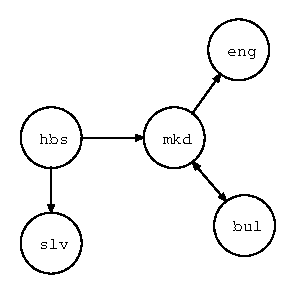
\includegraphics[width=0.2\textwidth]{images/south-slavic-apertium}
\caption{Language pairs including the South-Slavic languages in Apertium: \texttt{mkd} = Macedonian,
\texttt{bul} = Bulgarian; \texttt{eng} = English.}
\label{fig:pairs}
\end{figure}

The greatest difficulties for our system are caused by the long phrases present 
and the loose and free word order in the South Slavic languages.
Because of that, in future we plan to put more effort into dealing with those problems.
We are aware of the fact that it is difficult to write transfer rules between the two sides,
and we intend to address that issue by first improving the coverage of our dictionaries.

After expanding the dictionaries, we intend to put more time into developing the Slovenian constraint grammar,
and improve transfer by taking into account wider context.

We intend to work on more Slavic language pairs, including Serbo-Croatian--Russian,
and improve our existing ones (see Figure~\ref{fig:pairs}), including Serbo-Croatian--Macedonian \cite{peradin12} using the 
resources and knowledge obtained by developing this language pair.

Finally, we will keep the resources up to date in regard to current
regional linguistic developments, in particular we will add the
Montenegrin language once the standard is completely agreed on.

%mention different word order, long phrases, difficult to write rules for
%improve coverage, disambiguation (esp. for slv) and transfer rules
%work on more Slavic language pairs (e.g. hbs-rus)
%backport improvements in the HBS components to hbs-mak
%keep up-to-date with latest politico-linguistic developments. Add in
% Montenegrin when the standard is agreed on.
%small timeframe, disambiguation and transfer rudimentary

\section{Conclusions}

This language pair was an encouraging take on a pair of closely
related South-Slavic languages, and represents a satisfying conclusion
to an MT chain of neighbouring languages (the pairs Serbo-Croatian--Macedonian 
and Macedonian--Bulgarian are also available in Apertium). While we are aware that it
is still in its infancy, and has many flaws, it is a valuable
free/open-source resource, and will serve as another solid ground for NLP
in this language group.

